%  !TeX  root  =  user_guide.tex

\chapter{QGIS Server}\label{label_qgisserver}
\index{WMS!QGIS Server}

% when the revision of a section has been finalized,
% comment out the following line:
% \updatedisclaimer

QGIS Mapserver это свободная реализация сервера WMS, совместимого со стандартом
WMS 1.3, которая кроме того имеет дополнительные возможности для тематического
картографирования. QGIS mapserver является написаным на С++ приложением FastCGI/CGI
(Common Gateway Interface), которое работает совместно с веб-сервером
(например, Apache или Lighttpd). Разработка сервера финансируется проектами
Orchestra ЕС, Sany и администрацией города Uster (Швейцария).

Он использует QGIS для отрисовки карты и ГИС-логики. Графическая подсистема
реализована при помощи библиотеки Qt, это же  позволило получить кроссплатформенность.
В отличие от других WMS-решений, QGIS Mapserver использует картографические
правила в SLD/SE и как язык конфигурирования сервера, и для описания пользовательских
картографических правил.

Кроме того, проект QGIS Mapserver предоставляет расширение <<Publish to Web>>
для QGIS, при помощи которого можно экспортировать текущие слои и символику
в проект для QGIS Mapserver (включая правила отображения в формате SLD).

Так как QGIS и QGIS mapserver используют одни и те же библиотеки визуализации,
карта, опубликованная в Интернет, выглядит точно так же, как и в настольной
ГИС. Модуль <<Publish to Web>> поддерживает базовую символику, более сложные
правила картографической визуализации задаются вручную. В качестве конфигурационных
файлов используется стандарт SLD и его расширения, таким образом, необходимо
знать только один стандартизированный язык, что значительно уменьшает сложность
создания карт для Интернет.

В следующих версиях руковдоства будет приведена инструкция по базовой
настройке сервера. В настоящее же время получить больше информации можно
по следующим ссылкам:

\begin{itemize}
\item \url{http://karlinapp.ethz.ch/qgis\_wms/}
\item \url{http://www.qgis.org/wiki/QGIS\_mapserver\_tutorial}
\item \url{http://linfiniti.com/2010/08/qgis-mapserver-a-wms-server-for-the-masses/}
\end{itemize}

\section{Пример установки на Debian Squeeze}

В этом разделе кратко описан процесс установки на Debian Squeeze. Бинарные
сборки существуют и для многих других операционных систем. Если вы скомпилировали
сервер WMS самостоятельно, обратитесь к ранее приведенным сайтам.

Кроме самой \qg и сервера WMS нужен еще и web-сервер, в нашем случае apache2.
Установить необходимые пакеты со всеми зависимостями можно при помощи
\usertext{aptitude} или \usertext{apt-get install}.

После установки необходимо убедиться, что и web-сервер, и сервер WMS работают
правильно.

Запустите web-сервер, выполнив команду \usertext{/etc/init.d/apache2 start}.
Откройте браузер и введите адрес: \url{http://localhost}. Если apache
запущен и работает правильно, в окне браузера отобразится текст <<It works!>>.

Теперь можно перейти к проверке работоспособности сервера WMS. Исполняемый
файл qgis\_mapserv.fcgi расположенный в \filename{/usr/lib/cgi-bin/qgis\_mapserv.fcgi}
является стандартным шаблоном WMS и отображает границы штатов США, как
показано на рисунке~\ref{fig:usa_wms}. Добавьте адрес \url{http://localhost/cgi-bin/qgis\_mapserv.fcgi}
к списку серверов WMS QGIS, как это описано в разделе~\ref{sec:ogc-wms-servers}.

\begin{figure}[ht]
\centering
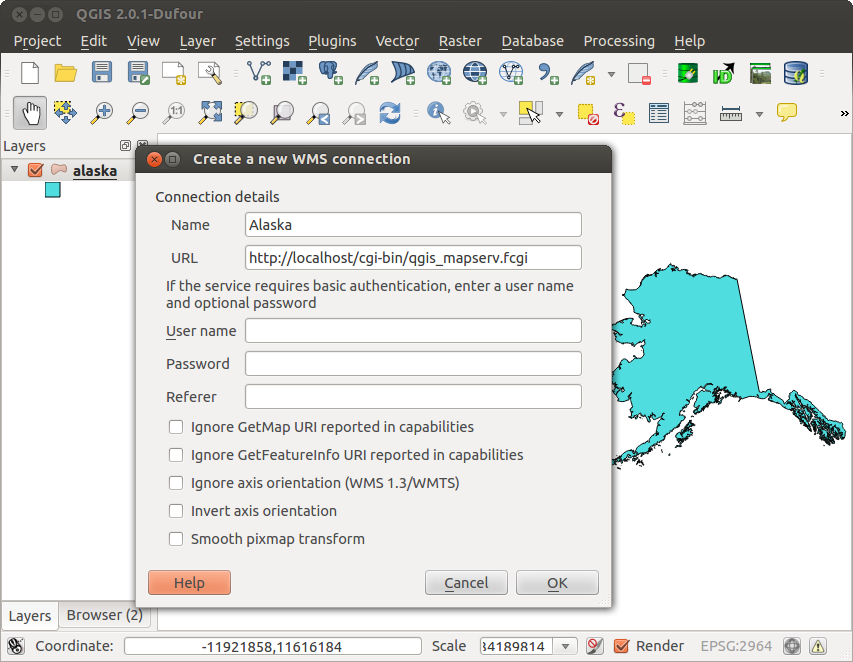
\includegraphics[clip=true, width=9cm]{standard_wms_usa}
\caption{Тестовый WMS с границами США из комплекта WMS сервера QGIS\nixcaption}
\label{fig:usa_wms}
\end{figure}

\section{Создание WMS на основе проекта QGIS}

Для создания нового сервера WMS нужно создать проект \qg и добавить в него
какие-то данные. В этом примере мы будем использовать shape-файлы <<regions>>
и <<aiport>> из демонстрационного набора данных \qg.

Сначала необходимо загрузить shape-файлы в проект, настроить цвета и стили
оформления слоёв, а также задать систему координат проекта. Затем вызовем
из меню \mainmenuopt{Установки} \arrow \mainmenuopt{Свойства проекта}
одноименное диалоговое окно и на вкладке \tab{Сервер WMS} заполним поля
<<Характеристики сервера>>, <<Достуные системы координат>> и <<Публикуемый
охват>>. При необходимости можно установить флажок
\checkbox{Включить WKT геометрию в ответ на GetFeatureInfo}, что сделает
возможным выполнение запросов к слою (см. Рисунок~\ref{fig:wmsdefinition}).
Сохраним проект как \filename{alaska\_airports.qgs}.

\begin{figure}[ht]
\centering
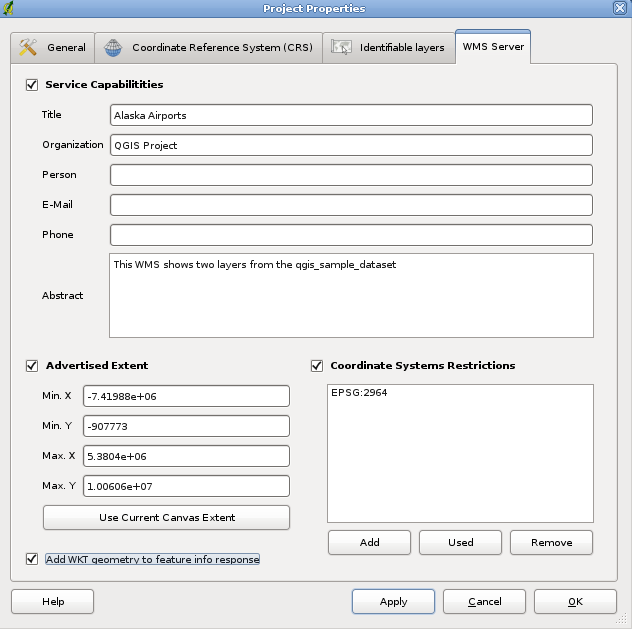
\includegraphics[clip=true, width=9cm]{wms_server_definition}
\caption{Характеристики проекта для сервера WMS \nixcaption}
\label{fig:wmsdefinition}
\end{figure}

Чтобы использовать сохраненный проект в качестве WMS, необходимо создать
новый подкаталог в каталоге \filename{/usr/lib/cgi-bin/project} (необходимы
привелегии суперпользователя), поместить в него файл проекта \filename{alaska\_airports.qgs}
и копию файла \filename{qgis\_mapserv.fcgi}.

Теперь можно проверить работу сервера, добавив его адрес
\url{http://localhost/cgi-bin/project/qgis\_mapserv.fcgi} в список серверов
WMS, как это описано в разделе~\ref{sec:ogc-wms-servers}. На рисунке~\ref{fig:wmsproject}
показана QGIS подключенная к серверу WMS на основе проекта.

\begin{figure}[ht]
\centering
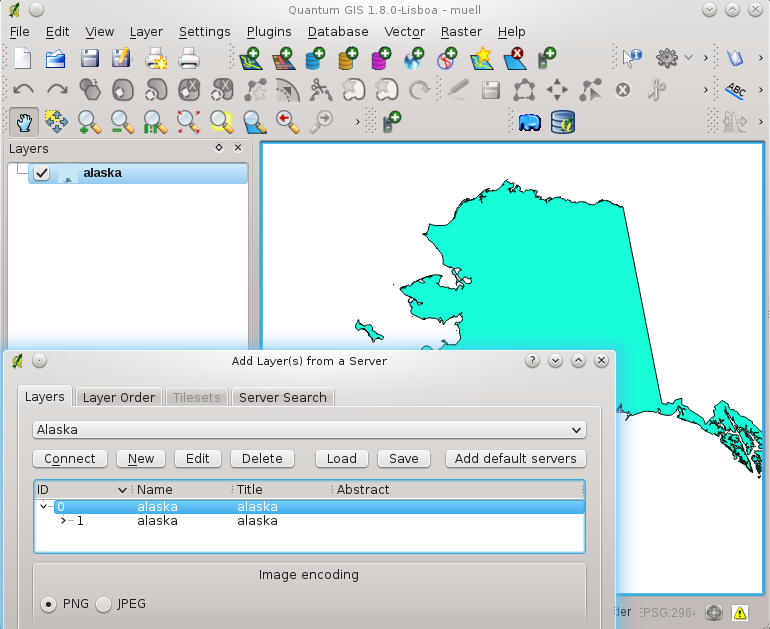
\includegraphics[clip=true, width=\textwidth]{wms_server_project}
\caption{Сервер WMS работающий на основе проекта QGIS \nixcaption}
\label{fig:wmsproject}
\end{figure}

\FloatBarrier
